\documentclass{beamer}
\mode<presentation>
\usepackage{amsmath}
\usepackage{amssymb}
%\usepackage{advdate}
\usepackage{adjustbox}
\usepackage{subcaption}
\usepackage{enumitem}
\usepackage{multicol}
\usepackage{mathtools}
\usepackage{listings}
\usepackage{url}
\usepackage{hyperref}
\def\UrlBreaks{\do\/\do-}
\usetheme{Boadilla}
\usecolortheme{lily}
\setbeamertemplate{footline}
{
  \leavevmode%
  \hbox{%
  \begin{beamercolorbox}[wd=\paperwidth,ht=2.25ex,dp=1ex,right]{author in head/foot}%
    \insertframenumber{} / \inserttotalframenumber\hspace*{2ex} 
  \end{beamercolorbox}}%
  \vskip0pt%
}
\setbeamertemplate{navigation symbols}{}

\providecommand{\nCr}[2]{\,^{#1}C_{#2}} % nCr
\providecommand{\nPr}[2]{\,^{#1}P_{#2}} % nPr
\providecommand{\mbf}{\mathbf}
\providecommand{\pr}[1]{\ensuremath{\Pr\left(#1\right)}}
\providecommand{\qfunc}[1]{\ensuremath{Q\left(#1\right)}}
\providecommand{\sbrak}[1]{\ensuremath{{}\left[#1\right]}}
\providecommand{\lsbrak}[1]{\ensuremath{{}\left[#1\right.}}
\providecommand{\rsbrak}[1]{\ensuremath{{}\left.#1\right]}}
\providecommand{\brak}[1]{\ensuremath{\left(#1\right)}}
\providecommand{\lbrak}[1]{\ensuremath{\left(#1\right.}}
\providecommand{\rbrak}[1]{\ensuremath{\left.#1\right)}}
\providecommand{\cbrak}[1]{\ensuremath{\left\{#1\right\}}}
\providecommand{\lcbrak}[1]{\ensuremath{\left\{#1\right.}}
\providecommand{\rcbrak}[1]{\ensuremath{\left.#1\right\}}}
\theoremstyle{remark}
\newtheorem{rem}{Remark}
\newcommand{\sgn}{\mathop{\mathrm{sgn}}}
\providecommand{\abs}[1]{\left\vert#1\right\vert}
\providecommand{\res}[1]{\Res\displaylimits_{#1}} 
\providecommand{\norm}[1]{\lVert#1\rVert}
\providecommand{\mtx}[1]{\mathbf{#1}}
\providecommand{\mean}[1]{E\left[ #1 \right]}
\providecommand{\fourier}{\overset{\mathcal{F}}{ \rightleftharpoons}}
%\providecommand{\hilbert}{\overset{\mathcal{H}}{ \rightleftharpoons}}
\providecommand{\system}{\overset{\mathcal{H}}{ \longleftrightarrow}}
	%\newcommand{\solution}[2]{\textbf{Solution:}{#1}}
%\newcommand{\solution}{\noindent \textbf{Solution: }}
\providecommand{\dec}[2]{\ensuremath{\overset{#1}{\underset{#2}{\gtrless}}}}
\newcommand{\myvec}[1]{\ensuremath{\begin{pmatrix}#1\end{pmatrix}}}
\let\vec\mathbf

\lstset{
%language=C,
frame=single, 
breaklines=true,
columns=fullflexible
}

\numberwithin{equation}{section}

\title{NCERT-11.16.3.11}
\author{Arnav Mahishi \\ Dept. of Electrical Engg.\\IIT Hyderabad.}

\date{\today} 
\begin{document}

\begin{frame}
\titlepage
\end{frame}
\section*{Outline}
\section{Problem}
\begin{frame}
\frametitle{Problem Statement}
In a lottery, a person chooses six different natural numbers at random from 1 to 20, and if these six numbers match with the six numbers aldready fixed by the lotttery committee, he wins a prize. What is the probability of winning the prize in the game?
\end{frame}
%\subsection{Literature}
\section{Solution}
\subsection{Theoritical Soln}
\begin{frame}
\frametitle{Theoritical Soln}
The sample space is 
\begin{align}
  \Omega &= \sbrak{\text{All possible collections of 6 numbers from 1 to 20}}\\
  \implies\abs{\Omega}&=\binom{20}{6}
\end{align}
Assuming equally likely outcomes, 
\begin{align}
  \Pr\brak{\omega \in \Omega} = \frac{1}{\abs{\Omega}}=\frac{1}{\binom{20}{6}}
\end{align}
\end{frame}
\subsection{CDF and PMF}
\begin{frame}
    \frametitle{CDF and PMF}
Let X represent the event:\newline
X=1, The person wins the prize (All the numbers match)\\
X=0: The person does not win (numbers don't match).\\
The Probability Mass Function (PMF) for the given random variable is
\begin{align}
P(X = k) =
\begin{cases}
	1-\frac{1}{\binom{20}{6}}, & k = 0 \\
	\frac{1}{\binom{20}{6}}, & k = 1 \\
\end{cases}
\end{align}
The Cumulative Distribution Function (CDF) for the given random variable is
\begin{align}
F_X(k) = P(X \le k) = 
\begin{cases}
	0, & k < 0 \\
	1-\frac{1}{\binom{20}{6}}, & 0 \le k < 1 \\
	1, & k \le 1\\
\end{cases}
\end{align}
The probability of winnig the lottery is
\begin{align}
  \Pr\brak{X=1} &= \frac{1}{\binom{20}{6}}
\end{align}
\end{frame}
\begin{frame}
\frametitle{Simulation}
To simulate the lottery the process follows these steps:\\
\textbf{Random Number Generation:} Generate random numbers uniformly from 1 to 20 for both the player and the committee using a uniform random number generator.\\
\textbf{Simulate Multiple Trials:} Run the simulation for a large number of trials (e.g., 1,000,000), where in each trial the player's six numbers are compared to the committee's six numbers.\\
\textbf{Match Calculation:} If all six numbers match, the player wins. The number of wins is tracked.\textbf{Probability Calculation:} Calculate the probability of winning as the ratio of winning trials to total trials. The true probability is \( \frac{1}{\binom{20}{6}} \)\\
\textbf{Relative Frequency:} Track and plot the relative frequency of winning over time to observe convergence to the true probability.
\end{frame}
\begin{frame}{Convergence of relative frequency to true probability}
\begin{figure}[h!]
   \centering
   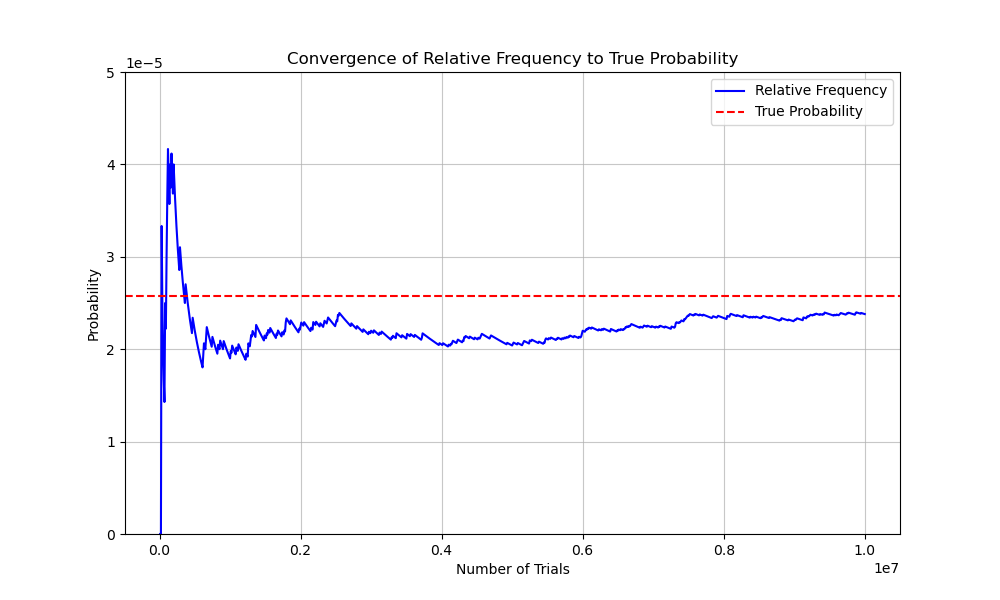
\includegraphics[width=0.7\columnwidth]{figs/fig.png}
    \caption{Relative Frequency tends to True Probability}
\end{figure}
\end{frame}
\begin{frame}{Probability Mass Function}
\begin{figure}[h!]
   \centering
   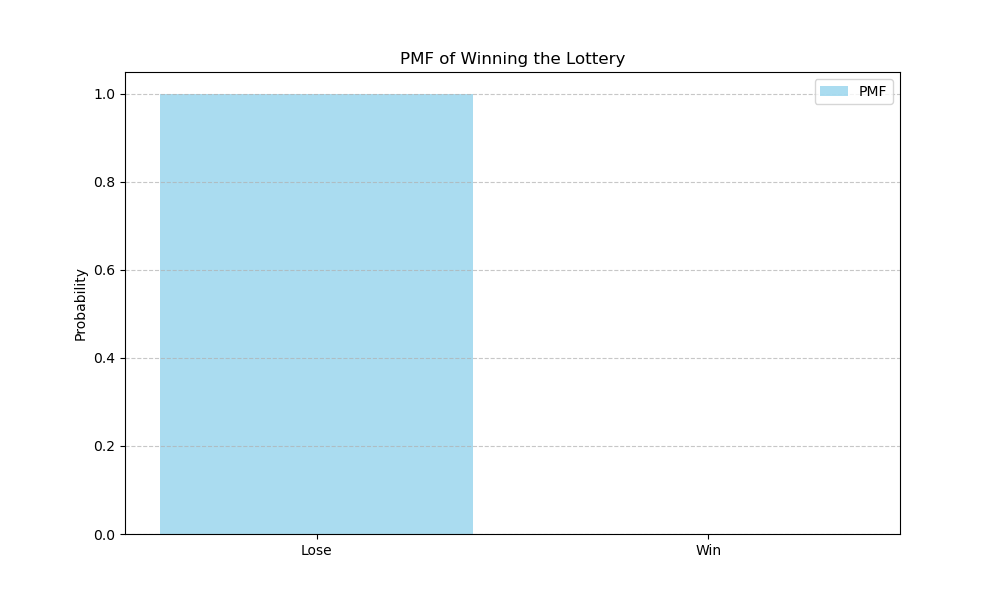
\includegraphics[width=0.7\columnwidth]{figs/pmf.png}
    \caption{Probability Mass Function of given Random variable}
\end{figure}
\end{frame}
\begin{frame}{Cumulative Distribution Function}
\begin{figure}[h!]
   \centering
   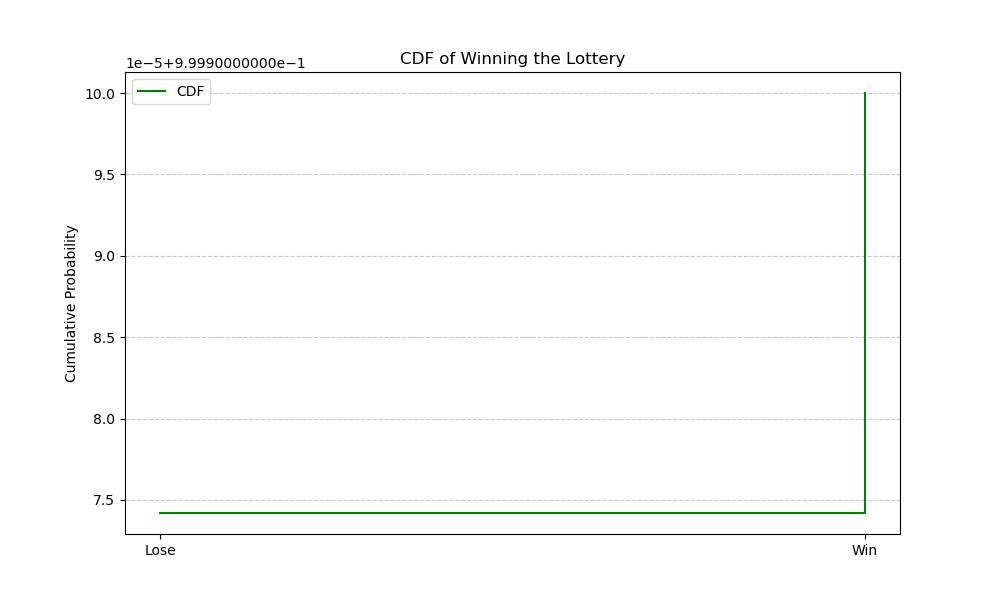
\includegraphics[width=0.7\columnwidth]{figs/cdf.png}
    \caption{Cumulative Distribution Function of given Random variable}
\end{figure}
\end{frame}
\end{document}
